
\paragraph{1. Preserving \textit{happens-before} relations}
        
        

    If $\stck{_{hb}}$ relations among events are lost after reordering, we may introduce new observable behaviors. The relations that are subject to change can be divided into four parts using events $e$ and $d$
    
    \begin{tasks}(2)
        \task $\reln{k}{hb}{e}$
        \task $\reln{e}{hb}{k}$
        \task $\reln{d}{hb}{k}$
        \task $\reln{k}{hb}{d}$ 
    \end{tasks}

    Firstly, note that the relations of the form $\reln{e}{hb}{k}$ come through either a $\stck{_{sw}}$ relation with $e$ or relations through event $d$, i.e. of the form $\reln{d}{hb}{k}$. The ones that come due to the latter, may not be preserved after reordering, if we strictly are only able to derive them with relations through $d$. Note also that, a similar argument exists for relations of the form $\reln{k}{hb}{d}$ wherein relations derived through $e$  ($\reln{k}{hb}{e}$) may be lost after reordering. 

    Hence, the relations that could be subject to change can be addressed by considering two disjoint sets of events in any \textit{Candidate Execution} of $C$ as below.
       
    \begin{align*}
       K_e = \{k \ | \ \reln{k}{hb}{e} \}. \\
       K_d = \{k \ | \ \reln{d}{hb}{k} \}. 
    \end{align*}
            
        %Show a figure here  (with Ke and Kd)
    \begin{figure}[H]
        \centering
        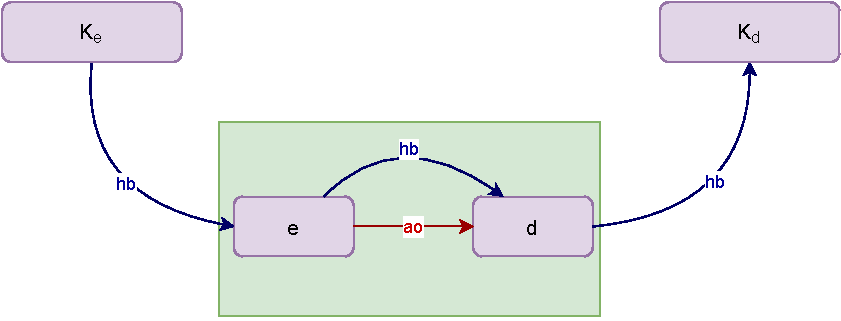
\includegraphics[scale=0.7]{InstructionReordering/ValidReorderingProof/ProofParts/Part1/part1(a).pdf}
        \caption{For any Candidate Execution of $C$, the set $K_e$ and $K_d$}
        \label{fig:my_label}
    \end{figure}
    
    Consider two events $\event{p1}{K_e}$ and $\event{p2}{K_d}$ (When $e$ is the first event or $d$ is the last event, assume dummyevents that can act as $p1$ or $p2$.) belonging to the same agent as that of $e$ and $d$ such that in $C$:
    \begin{align*}
        dir(p1,e)\ \wedge\ dir(d,p2).
    \end{align*}
    
    Note that in terms of direct happens-before relations, on reordering, any $Candidate Execution$ of $C$ will have the followingchanges
    %Show a figure here 
    \begin{figure}[H]
        \centering
        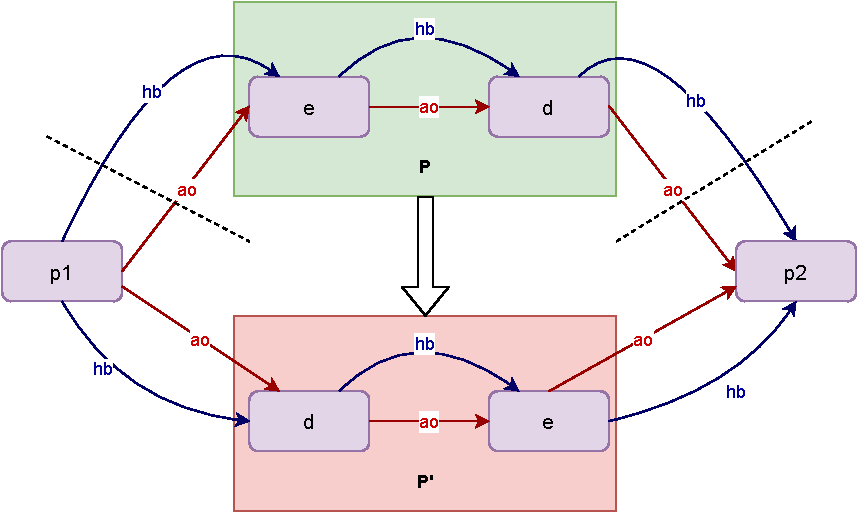
\includegraphics[scale=0.7]{InstructionReordering/ValidReorderingProof/ProofParts/Part1/part1(b).pdf}
        \caption{The direct relation changes that can be observed while reordering events $e$ and $d$}
        \label{fig:my_label}
    \end{figure}
    
    The figure above is to show that, for any $Candidate Execution$ of $C$, the following is true
    \[
        cons(p1,e) \ \wedge dir(p1,e) \ \wedge dir(e,d) \ \wedge cons(d,p2) \ \wedge \ dir(d,p2).
    \]
    and for that of $C'$,
    \[
        cons(p1,d) \ \wedge \ dir(p1,d) \ \wedge \ dir(d,e) \ \wedge cons(e,p2) \ \wedge dir(e,p2).
    \]
    
    We need the following key relations to be preserved in Candidate executions of $C'$ 
    \begin{tasks}(2)
        \task $\reln{p1}{hb}{e}$
        \task $\reln{e}{hb}{k}$
        \task $\reln{d}{hb}{p2}$
        \task $\reln{k}{hb}{d}$ 
    \end{tasks}

    After reordering, we do have these relations preserved due to transitivity  
    \begin{gather*}
        \reln{p1}{hb}{d} \ \wedge \ \reln{d}{hb}{e} \ \Rightarrow \ \reln{p1}{hb}{e}. \\
        \reln{e}{hb}{p2} \ \wedge \ \reln{d}{hb}{e} \ \Rightarrow \ \reln{d}{hb}{p2}. \\
        \reln{p1}{hb}{d} \ \wedge \ \reln{d}{hb}{e} \ \wedge \ \reln{e}{hb}{p2} \ \Rightarrow \ \reln{p1}{hb}{p2}. 
    \end{gather*}

    The other two forms of relations may not be preserved due to $\reln{d}{sw}{k}$ or $\reln{k}{sw}{d}$. If we can "pivot" the  set $K_e$ to $p1$ and $K_d$ to $p2$, it would ensure that our other two intended relations also remain preserved after reordering by transitivity. To state formally, we have a valid pair of pivots $<p1,p2>$ when the following two conditions hold
    \begin{gather*}
        \forall \ k \in K_e - \{p1\}, \ \reln{k}{hb}{p1}. \\
        \forall \ k \in K_d - \{p2\}, \ \reln{p2}{hb}{k}.
    \end{gather*}
    
    %Show a figure here
    \begin{figure}[H]
        \centering
        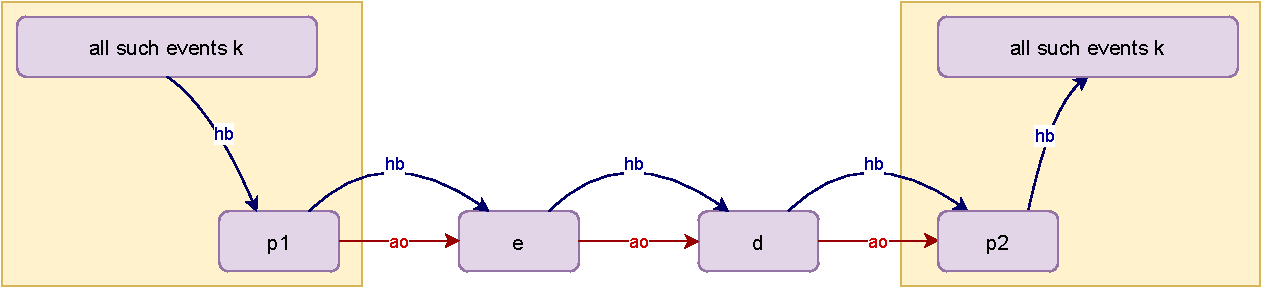
\includegraphics[scale=0.7]{InstructionReordering/ValidReorderingProof/ProofParts/Part1/part1(d).pdf}
        \caption{For any Candidate execution, the intuition behind valid pivots $<p1,p2>$}
        \label{fig:my_label}
    \end{figure}
    
    By lemma 1 and lemma 2 respectively, we have for $C$, the following condition where $<p1, p2>$ is a valid pivot pair
    \begin{gather*}
        \et{e}{uo} \vee (\et{e}{sc} \wedge \event{e}{W}). \\
        \et{d}{uo} \vee (\et{d}{sc} \wedge \event{d}{R}).
    \end{gather*}
        
    The following table summarizes the cases where we have a valid pair of pivots $<p1,p2>$
    %Show a general table here 
    \begin{figure}[H]
        \centering
        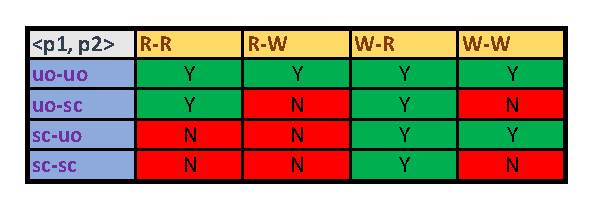
\includegraphics[scale=0.7]{InstructionReordering/ValidReorderingProof/ProofParts/Part1/part1_table.pdf}
        \caption{Table summarizing whether we have valid pair of pivots based on  $e$ and $d$}
        \label{fig:my_label}
    \end{figure}
            
    We show a simple example where we do not have a valid pair of pivots, particularly because $p1$ is not a valid pivot. Note thatin this example, $K_e = K_{e1} + K_{e2} + p1 + p_x$
    %Show figure here of program P
    \begin{figure}[H]
        \centering
        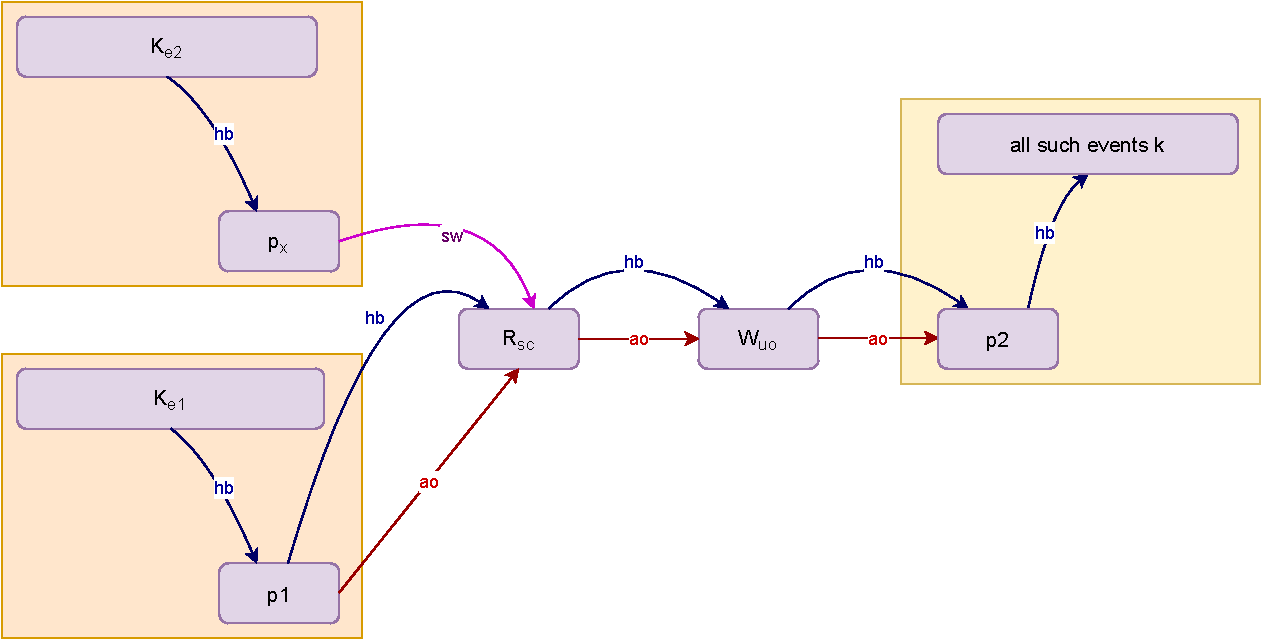
\includegraphics[scale=0.7]{InstructionReordering/ValidReorderingProof/ProofParts/Part1/part1(e).pdf}
        \caption{A Candidate Execution where p1 is not a valid pivot}
        \label{fig:my_label}
    \end{figure}
    
    %Show figure here of program P'
    \begin{figure}[H]
        \centering
        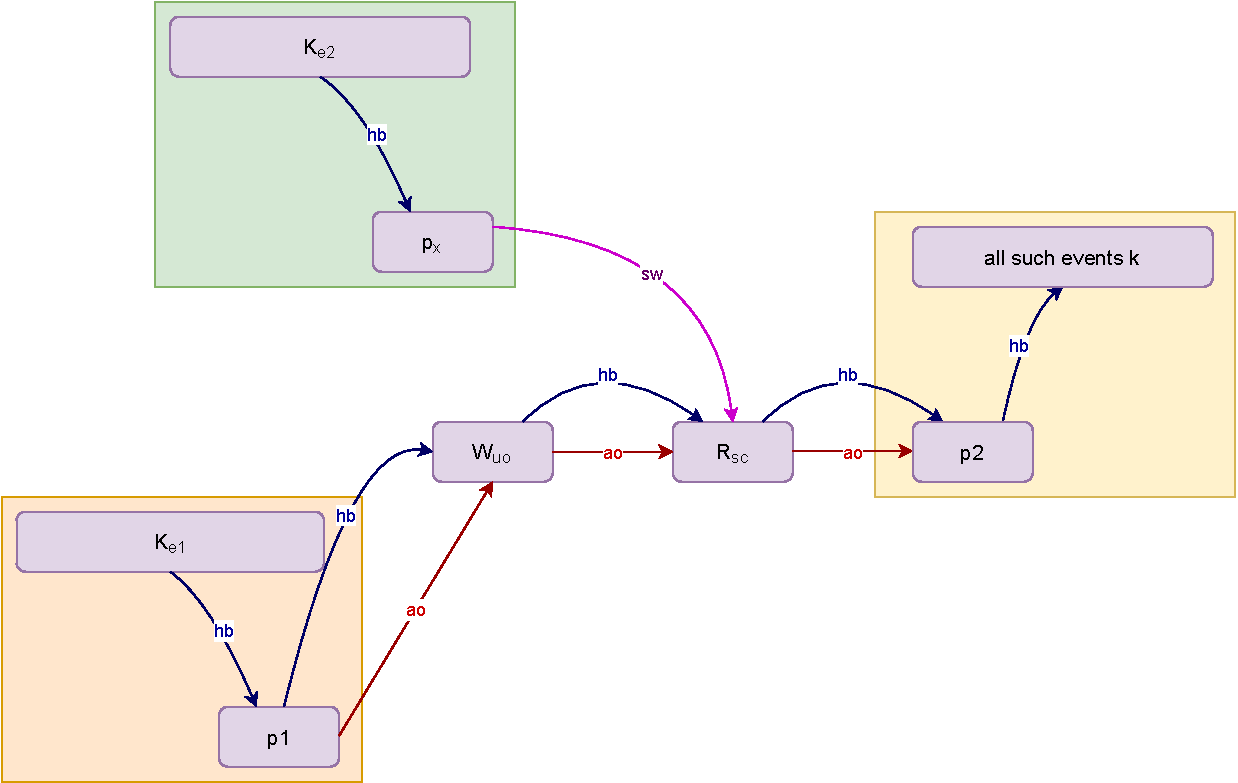
\includegraphics[scale=0.7]{InstructionReordering/ValidReorderingProof/ProofParts/Part1/part1(f).pdf}
        \caption{The resultant Candidate Execution after reordering, exposing the relations with $p_x$, $K_{e2}$ and $d$ that arelost}
        \label{fig:my_label}
    \end{figure}
        
    \critic{purple}{Strictly speaking, it is not that the happens-before relations are preserved, but that the properties between different happens before relations hold, which implies that for any possible Candidate Execution after reordering, the set of happens-before relatiosn apart from that between $e$ and $d$ remain the same. I am emphasizing this point because we view reordering as just changing agent order between two events, which just needs information from Candiadate but not all its possible Executions.}